\documentclass[conference]{IEEEtran}

\usepackage{amsmath,amssymb}
\usepackage{booktabs}
\usepackage{graphicx}
\usepackage{microtype}
\usepackage{xcolor}

\graphicspath{{figures/}}

\title{Accuracy Retention Is Not Explanation Retention:\\
Physiological Explanation Drift in Continual EEG Foundation Models}

\author{\IEEEauthorblockN{Author Name(s)---replace before submission}
\IEEEauthorblockA{Affiliation and contact---replace before submission}}

\begin{document}
\maketitle

\begin{abstract}
Continual adaptation can preserve an EEG decoder's accuracy while changing the
evidence behind its decisions. We study this failure mode in CBraMod across
motor-imagery, motor-execution/rest, and sleep-staging tasks. We define
channel--frequency reliance by the class-balanced drop in true-vs-best-other
classification margin after single-cell spectral occlusion. Before measuring
drift, we require subject-level split-half reliability and held-out
top-vs-random fidelity. Physiological explanation drift (PED) is then the
symmetric cross-checkpoint Jensen--Shannon divergence minus same-checkpoint
split noise. Across three task orders, three seeds, and 63 old-task transitions,
sequential fine-tuning exhibits substantial PED even when old-task accuracy
improves. EWC and DER++ reduce PED relative to matched sequential runs in all
21 comparisons; order--seed-blocked mean reductions are $-0.122$ and $-0.080$,
respectively. Yet within-method correlations between relative forgetting and
PED remain weak ($\rho=-0.37, 0.09, -0.21$). Thus, performance retention alone
does not establish physiological explanation stability in continual EEG
foundation models.
\end{abstract}

\begin{IEEEkeywords}
EEG foundation models, continual learning, explainable AI, attribution
stability, catastrophic forgetting
\end{IEEEkeywords}

\section{Introduction}
EEG foundation models (EEG-FMs) offer a shared representation for heterogeneous
clinical and brain--computer-interface tasks~\cite{wang2025cbramod}. Their
downstream lifetime, however, is usually assessed through predictive
performance: after learning a new task, does the model still classify an old
task correctly? Recent continual EEG work, including EvoBrain, directly targets
this stability--plasticity problem~\cite{zhou2026evobrain}. Accuracy does not
reveal whether the model still uses the same physiological evidence.

Explanation drift has been studied in generic continual-learning benchmarks.
CLEX showed that similarly accurate models can produce different explanations,
and that replay can improve alignment with offline models~\cite{cossu2024clex}.
SHAP consistency provides a related attribution-stability view on vision
benchmarks~\cite{cai2024shapc}. Separately, static EEG-FM audits recover
task-appropriate spatial or spectral structure~\cite{sirca2026beyond,tang2026capture},
while EEG-PRISM maps attribution into physiologically meaningful frequency and
source domains~\cite{shama2026prism}. The intersection remains unresolved:
does physiologically structured evidence remain stable throughout cross-task
continual EEG-FM adaptation?

We ask two questions. \emph{RQ1:} how much does an old task's channel--frequency
reliance change after a task transition? \emph{RQ2:} do methods that reduce
performance forgetting also preserve explanations, and is retained accuracy a
reliable proxy for explanation stability? Our contributions are:
\begin{itemize}
    \item a reliability- and fidelity-gated channel--frequency reliance
    instrument based on held-out spectral occlusion and classification margins;
    \item a subject-level, noise-corrected PED estimator that separates
    cross-checkpoint change from same-checkpoint split variability; and
    \item a matched comparison of sequential fine-tuning, EWC, and DER++ over
    27 continual runs, showing that aggregate performance and explanation
    retention can improve together while transition-level accuracy remains an
    unreliable proxy for explanation stability.
\end{itemize}

\begin{figure*}[t]
    \centering
    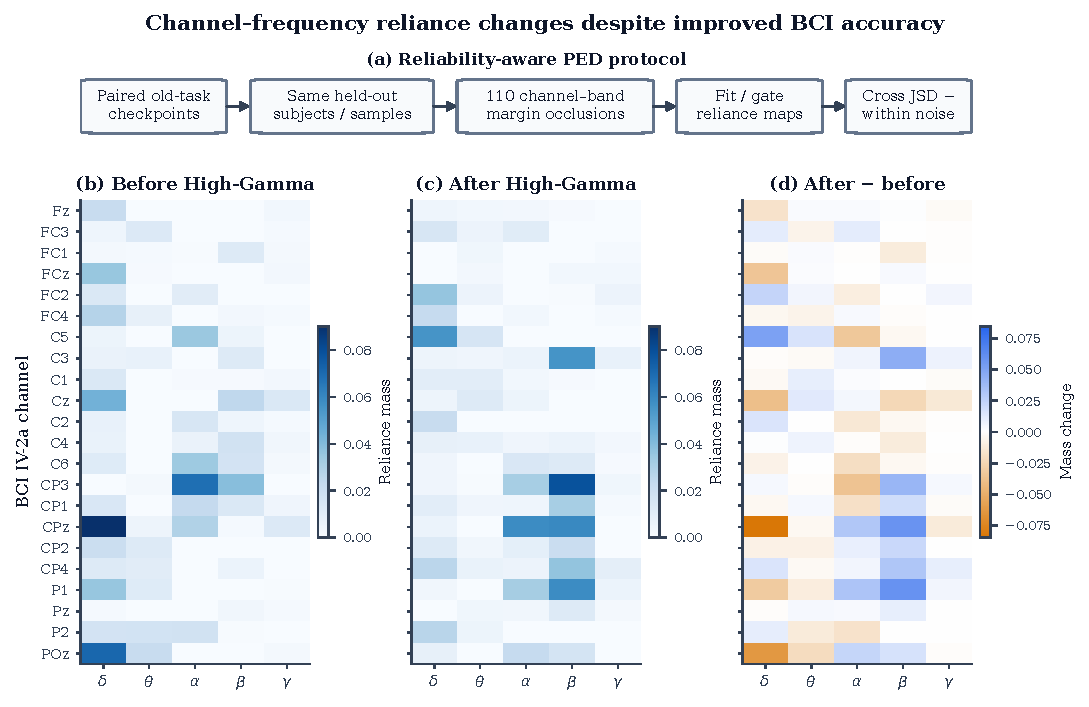
\includegraphics[width=\textwidth]{figure1_protocol_maps.pdf}
    \caption{PED protocol and BCI IV-2a reliance before/after learning
    High-Gamma. Maps average positive-normalized group reliance over three
    forward-order seeds; they are not selected from a single favorable run.
    BCI accuracy improves on average ($F_{rel}=-0.255$), although the
    channel--frequency distribution changes substantially (PED $=0.243$).}
    \label{fig:protocol}
\end{figure*}

\section{Reliability-Aware Explanation Drift}
\subsection{Channel--frequency reliance}
For task $i$, let $m(x)$ be the true-class logit minus the largest competing
logit. Each continuous trial is transformed by rFFT and one channel--band cell
is set to zero before inverse rFFT. We use 22 canonical channels and five bands:
$[0.5,4)$, $[4,8)$, $[8,13)$, $[13,30)$, and $[30,40]$~Hz. Reliance is
the decrease in margin caused by the occlusion, averaged first within class,
then equally across classes and subjects. Validation rows are deterministically
split within each subject/class into attribution-fit and attribution-gate
halves. Test rows are never used for attribution.

An attribution instrument must pass two gates before scale. Reliability requires
finite split-half cosine similarity, median subject cosine at least $0.70$, and
at least two thirds of subjects above $0.50$. Fidelity selects the top 20\%
cells on the fit half and requires both margin and subject-balanced-accuracy
drops on the gate half to exceed the 95th percentile of 100 equal-cardinality
random masks. BCI passes reliability (subject cosines $0.923/0.804$) and
fidelity. High-Gamma passes with median cosine $0.992$ (4/4 subjects above
$0.50$); its margin fidelity is clear ($1.801>1.594$), whereas BA fidelity is
narrow ($0.2563>0.2553$). Sleep attribution is excluded because it is reliable
but fails fidelity.

\subsection{Noise-corrected PED}
Let $P^{b}_{f},P^{b}_{g},P^{a}_{f},P^{a}_{g}$ be positive, $\ell_1$-normalized
reliance maps before/after a transition, on the fit/gate halves. For each
subject, we define
\begin{align}
\mathrm{PED} =&\ \tfrac12\!\left[\mathrm{JSD}(P^{b}_{f},P^{a}_{g})+
\mathrm{JSD}(P^{b}_{g},P^{a}_{f})\right] \nonumber\\
&-\tfrac12\!\left[\mathrm{JSD}(P^{b}_{f},P^{b}_{g})+
\mathrm{JSD}(P^{a}_{f},P^{a}_{g})\right].
\label{eq:ped}
\end{align}
Negative estimates are retained. Performance forgetting is
$F_{rel}=(R_{before}-R_{after})/(R_{before}-R_{chance})$; near-chance
denominators are reported as invalid rather than clipped.

\section{Experimental Protocol}
We fine-tune CBraMod~\cite{wang2025cbramod} with a shared backbone and a frozen
head for each old task. The replacement matrix contains BCI Competition IV-2a
(4-class motor imagery, 22 channels, 9 subjects), High-Gamma
(4 motor-execution/rest classes, 22 of 128 channels, 14 subjects)~\cite{schirrmeister2017},
and Sleep-EDF Expanded (5-stage sleep classification, two bipolar channels, 78
subjects)~\cite{sleepedf}. Signals are resampled to 200~Hz, restricted to
0.5--40~Hz, and represented as 1-s patches; High-Gamma uses 4-s trials and
Sleep uses 30-s epochs. Subject splits are fixed at 5/2/2, 7/4/3, and 48/15/15
for train/validation/test.

We compare sequential fine-tuning, offline EWC~\cite{kirkpatrick2017ewc} with
$\lambda=10^5$, and DER++~\cite{buzzega2020der} with an 8-MiB reservoir (119
items). Hyperparameters are selected once on validation data and reused.
Every task receives 2,500 optimizer steps with the final four encoder blocks
plastic. Three task orders and seeds $\{3407,42,2026\}$ produce 27 runs. PED is
evaluated for old BCI and High-Gamma tasks only, yielding 21 transition cells
per method (63 total). Statistical comparisons average transitions within each
of nine order--seed blocks, then use a 20,000-replicate block bootstrap and a
two-sided sign test. Transition-cell Spearman correlations are descriptive
because cells share orders, seeds, and subjects.

\begin{figure*}[t]
    \centering
    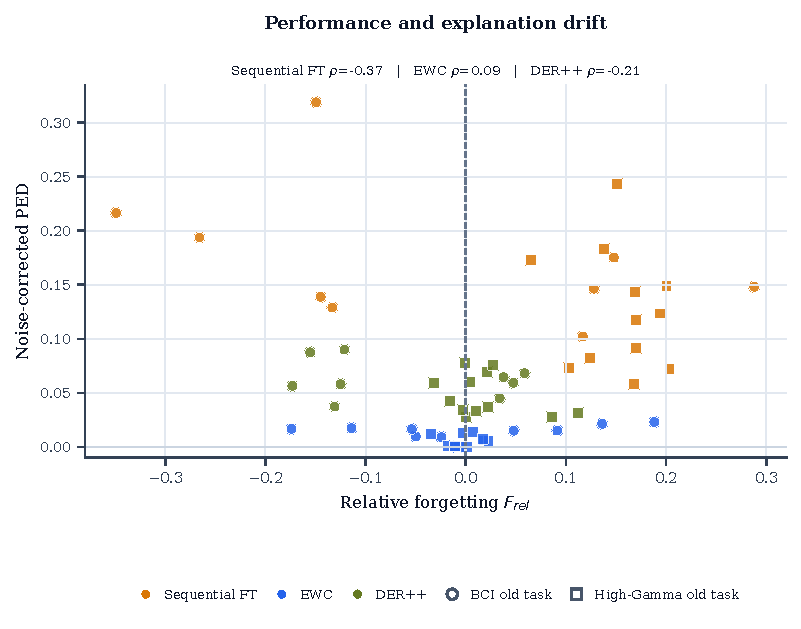
\includegraphics[width=0.513\textwidth]{figure2a_performance_ped.pdf}
    \hfill
    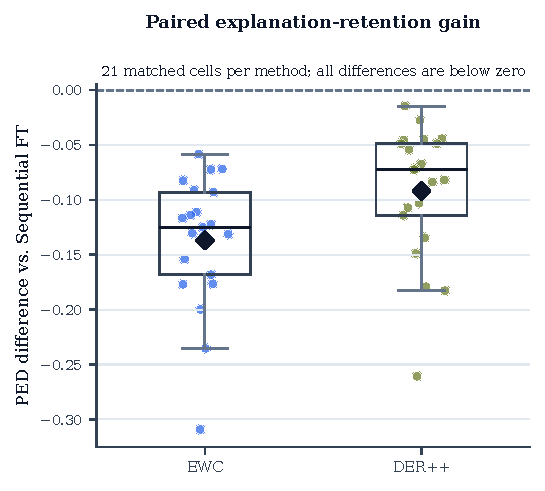
\includegraphics[width=0.447\textwidth]{figure2b_paired_ped.pdf}
    \caption{Performance--explanation alignment. (a) Each point is one matched
    order--seed--transition cell; color denotes method and marker denotes the
    old task. (b) Paired PED difference relative to sequential fine-tuning;
    diamonds show means. Both EWC and DER++ reduce PED in all 21 matched cells.}
    \label{fig:results}
\end{figure*}

\begin{table*}[t]
\centering
\caption{Performance forgetting and subject-level noise-corrected PED (mean $\pm$ SD across matched order--seed transition cells). Lower is better; negative $F_{rel}$ denotes backward transfer.}
\label{tab:main}
\setlength{\tabcolsep}{3.2pt}
\begin{tabular}{lrrrrrr}
\toprule
& \multicolumn{2}{c}{Sequential FT} & \multicolumn{2}{c}{EWC} & \multicolumn{2}{c}{DER++} \\
Direction & $F_{rel}$ & PED & $F_{rel}$ & PED & $F_{rel}$ & PED \\
\midrule
BCI$\leftarrow$High-$\gamma$ & -0.255 $\pm$ 0.100 & 0.243 $\pm$ 0.067 & -0.113 $\pm$ 0.062 & 0.015 $\pm$ 0.004 & -0.070 $\pm$ 0.101 & 0.052 $\pm$ 0.012 \\
BCI$\leftarrow$Sleep & 0.067 $\pm$ 0.171 & 0.140 $\pm$ 0.024 & 0.064 $\pm$ 0.093 & 0.017 $\pm$ 0.005 & -0.053 $\pm$ 0.108 & 0.069 $\pm$ 0.018 \\
High-$\gamma$$\leftarrow$BCI & 0.156 $\pm$ 0.036 & 0.082 $\pm$ 0.020 & -0.009 $\pm$ 0.006 & 0.0003 $\pm$ 0.0002 & 0.036 $\pm$ 0.051 & 0.033 $\pm$ 0.006 \\
High-$\gamma$$\leftarrow$Sleep & 0.153 $\pm$ 0.049 & 0.169 $\pm$ 0.042 & 0.004 $\pm$ 0.021 & 0.010 $\pm$ 0.004 & 0.003 $\pm$ 0.021 & 0.063 $\pm$ 0.016 \\
\bottomrule
\end{tabular}
\end{table*}


\section{Results}
\subsection{Performance retention does not imply explanation retention}
Sequential fine-tuning changes explanations in every direction
(Table~\ref{tab:main}). The clearest decoupling is
BCI$\leftarrow$High-Gamma: BCI performance improves
($F_{rel}=-0.255\pm0.100$), while PED remains the largest observed
($0.243\pm0.067$; Fig.~\ref{fig:protocol}). Therefore, a favorable backward
transfer score does not establish that the old decision rule was preserved.
Across the 21 cells, forgetting and PED are weakly associated within each
method: Spearman $\rho=-0.370$ for sequential fine-tuning, $0.088$ for EWC,
and $-0.214$ for DER++. These associations are exploratory and do not support
a causal relation.

\subsection{EWC and DER++ preserve explanations beyond accuracy}
EWC reduces subject-level PED relative to matched sequential runs in 21/21
cells, as does DER++ (Fig.~\ref{fig:results}). After averaging transitions
within each order--seed block, EWC's mean PED reduction is $-0.122$ (95\%
bootstrap CI $[-0.148,-0.095]$); DER++'s is $-0.080$
($[-0.103,-0.058]$). Both improve in 9/9 blocks (two-sided sign-test
$p=0.0039$). EWC is strongest: mean PED ranges from $0.0003$ to $0.0167$
across directions, compared with $0.0333$--$0.0687$ for DER++ and
$0.0825$--$0.2431$ for sequential fine-tuning. Thus, the CL methods improve
both performance and explanation retention in aggregate, but only direct PED
measurement reveals the stability of individual transitions.

\section{Limitations and Conclusion}
The study uses one backbone, three task orders, three seeds, and small BCI and
High-Gamma test cohorts. High-Gamma includes overt movement/rest and may contain
movement or EMG confounds; it is not treated as pure motor imagery. Its BA
fidelity gate passes by only $0.0010$. Old-task Sleep explanations are excluded
after a predeclared fidelity failure, so physiological claims cover BCI and
High-Gamma only. High-Gamma was introduced as a locked replacement after a
PhysioNet attribution gate failed, which should be considered when assessing
dataset-selection risk. PED measures post-hoc attribution stability, not a
biological engram or a causal mechanism of forgetting. We also do not establish
alignment with a unique offline explanation.

Within these limits, the evidence is consistent: EWC and DER++ preserve
channel--frequency reliance far better than sequential fine-tuning, yet accuracy
alone cannot identify whether an individual transition preserves the model's
physiological decision basis. Continual EEG-FM evaluation should therefore
report explanation retention alongside performance retention.

\clearpage
\bibliographystyle{IEEEtran}
\bibliography{references}

\end{document}
